\chapter{\topos{}的内语言}

\philoquote{
    A mathematical statement is just a story you tell about some devices. Some of those stories are clever, some are stupid; some of those stories are true, some others are false. Doing mathematics is telling clever stories which are true.\footnotemark
}{
    Francis Borceux, \cite{HCA3}
}
\footnotetext{一句数学陈述不过是你对某些东西讲的一个故事. 这些故事有的妙, 有的蠢, 有的真, 有的假. 做数学就是要讲出又妙又真的故事.}

\minitoc

我们曾提到\topos{}中有一种\emph{内语言} (internal language) 可用来进行推理, 本章介绍这种语言, 以及它在各个数学分支中的应用.

\begin{remark}
	{}
	建议读者在阅读本章之前先阅读附录 \ref{logic-appendix}.
\end{remark}

\section{Mitchell--B\'enabou 语言}

\label{Mitchell--Benabou-language}

本节描述一种重要的语言, 称作 \emph{Mitchell--B\'enabou 语言}; 它是由给定的\topos{} $\mathcal C$ 定义出的一种一阶或高阶语言, 其特点是利用子对象分类器 $\Omega$, 将\emph{公式}一视同仁地解释为 $\Omega$ 类型的\emph{项}. 使用这种语言, 可将\topos{}中的对象在语法上当作集合一样处理.

\begin{definition}
    {(类型)}
    Mitchell--B\'enabou 语言中的\emph{类型}是 $\mathcal C$ 的对象.
\end{definition}


%\begin{itemize}
%	\item 类型 $X$ 的\emph{项}被解释为指向 $X$ 的态射, 而\emph{公式}被解释为 $\Omega$ 类型的项;
%	项 (公式) 的定义域代表此项 (公式) 中自由变量的类型.
%	例如, 当类型 $X$ 的一个项含有自由变量 $y\colon Y, z\colon Z$ 时, 该项解释为一个态射 $Y\times Z \to X$.
%	\item 
%	\item 
%\end{itemize}


\begin{definition}
	{(函数符号, 关系符号)}
	Mitchell--B\'enabou 语言中的\emph{函数符号} $f\colon A_1\cdots A_n \to B$ 是 $\mathcal C$ 中的态射
	$$f\colon A_1\times\cdots\times A_n\to B.$$
	特别地, 类型 $X$ 的\emph{常量} (零元函数) 是态射 $1 \to X$, 也即对象 $X$ 的\emph{整体元素}.
	
	Mitchell--B\'enabou 语言中的\emph{关系符号} $R\hookrightarrow A_1\cdots A_n$ 是 $\mathcal C$ 中的态射
	$$
	R\colon A_1\times\cdots\times A_n \to \Omega,
	$$
	也即 $A_1\times\cdots\times A_n$ 的子对象, 其直观为 ``满足关系 $R$ 的元素构成的子集''.
	特别地, 原子命题 (零元关系) 是态射 $1\to\Omega$, 也即\emph{真值}.
	
	%我们看到, 函数符号与项被解释成了同一种东西. 这是有道理的, 因为\emph{项}在这里就是其自由变量的函数.
\end{definition}

% 至此, Mitchell--B\'enabou 语言已经定义完成.

以上两个定义给出了一个符号表 $\Sigma$, 自然, $\mathcal C$ 中具有典范的 $\Sigma$-结构.
由定义 \ref{term-interpretation}, \ref{higher-order-term-interpretation}, 可以归纳地得到所有项和公式的\emph{解释} (interpretation).
注意在附录 \ref{logic-appendix} 中公式被解释为子对象, 而在\topos{}中它等同于类型 $\Omega$ 的项.

%\begin{definition}
%    {(变量的解释)}
%    
%\end{definition}


%\begin{definition}
%	{(等式)}
%	
%\end{definition}


%\begin{propdef}
%	{(项的解释)}
%	类型 $X$ 的项解释为指向 $X$ 的态射 $\sigma\colon U\to X$, 其中 $U$ 是该项所含的变量的类型.
%	\begin{itemize}
%		\item (变量)
%		类型 $X$ 的一个\emph{变量} (可视为含一个自由变量的项) $x\colon X$ (为了体现与集合论的相似性也记为 $x\in X$) 解释为恒等态射 $\operatorname{id}\colon X \to X$.
%		\item (函数取值)
%		对于函数符号 $f\colon X \to Y$ 与类型 $X$ 的项 $\sigma\colon U \to X$, $f(\sigma)$ 解释为复合 $f\circ\sigma \colon U \to Y$.
%	\end{itemize}
%	由 (一阶语言中) 项的定义 (\ref{definition-terms}), 上述条款归纳地解释了所有的项.
%	高阶语言的项还需要如下的解释.
%	\begin{itemize}
%		\item (二元对, )
%		\item ()
%		\item (函数引入法则, 即 ``$\lambda$-演算'') 设 $x$ 是类型 $X$ 的变量, $\sigma\colon X\times U\to Z$ 是任意项,
%		那么 $\lambda x.\sigma$ 解释为 $\sigma$ 在伴随之下对应的态射 $U\to Z^X$.
%		\item (函数消去法则) 对于
%	\end{itemize}
%\end{propdef}

\begin{example}
	{(变量, 一般元素)}
	设 $x$ 是类型 $X$ 的一个变量. 由定义 \ref{term-interpretation}, 其解释为 $\operatorname{id}\colon X\to X$.
	
	变量 $x$ 可视为类型 $X$ 的\emph{一般元素} (generic element).
	其中 ``元素'' 是指广义元素, 即指向 $X$ 的态射; ``一般'' 是指如下的泛性质: 假若我们证明了含变量 $x$ 的公式 $\phi(x)$,
	那么对 $X$ 的任意具体的项 (广义元素) $x_0\colon U\to X$, 都有 $\phi(x_0)$ 成立.
	这是由于 $\operatorname{id}_X$ 是所有指向 $X$ 的态射中的终对象.
\end{example}

\begin{example}
	{(函数的取值)}
	使用取值映射 $\operatorname{ev}\colon Y^X\times X\to Y$ (定义 \ref{evaluation-map}),
	可将 $Y^X$ 类型的项 (内语言中的 ``函数'') $\theta\colon V\to Y^X$
	作用于 $X$ 类型的项 $\sigma \colon U \to X$,
	得到 $Y$ 类型的项
	% https://q.uiver.app/#q=WzAsMyxbMCwwLCJWXFx0aW1lcyBVIl0sWzEsMCwiWV5YXFx0aW1lcyBYIl0sWzIsMCwiWSJdLFswLDEsIihcXHRoZXRhLFxcc2lnbWEpIl0sWzEsMiwiXFxvcGVyYXRvcm5hbWV7ZXZ9Il1d
	\[\theta(\sigma)\colon
	\begin{tikzcd}[ampersand replacement=\&]
		{V\times U} \& {Y^X\times X} \& Y.
		\arrow["{(\theta,\sigma)}", from=1-1, to=1-2]
		\arrow["{\operatorname{ev}}", from=1-2, to=1-3]
	\end{tikzcd}\]
\end{example}

\begin{example}
	{(成员关系)}
	考虑成员关系 (例 \ref{membership-relation}) ${\in_X} \colon \Omega^X\times X \to \Omega$,
	可对 $PX=\Omega^X$ 类型的项 (内语言中的 ``子集'') $\eta\colon V \to \Omega^X$ 与 $X$ 类型的项 $\sigma\colon U\to X$ 定义 $\Omega$ 类型的项
	% https://q.uiver.app/#q=WzAsMyxbMCwwLCJWXFx0aW1lcyBVIl0sWzEsMCwiXFxPbWVnYV5YXFx0aW1lcyBYIl0sWzIsMCwiXFxPbWVnYSJdLFswLDEsIihcXGV0YSxcXHNpZ21hKSJdLFsxLDIsIlxcaW5fWCJdXQ==
	\[
	(\sigma \in \eta) \colon 
	\begin{tikzcd}[ampersand replacement=\&]
		{V\times U} \& {\Omega^X\times X} \& \Omega.
		\arrow["{(\eta,\sigma)}", from=1-1, to=1-2]
		\arrow["{\in_X}", from=1-2, to=1-3]
	\end{tikzcd}\]
\end{example}

\begin{example}
	{(等式)}
	对于类型 $X$ 的变量 $x_1,x_2$, \emph{等式} $x_1 = x_2$ 被解释为 $\chi_\Delta\colon X\times X\to\Omega$, 即对角线 $\Delta\colon X\to X\times X$ 的特征函数 (例 \ref{diagonal}).
\end{example}

\begin{example}
	{(存在量词与任意量词)}
	设 $\phi(x,y)$ 是含两个变量 $x\in X,y\in Y$ 的公式.
		考虑投影 $\pi\colon X\times Y\to Y$ 诱导的子对象偏序集之间的三元伴随
		\[\begin{tikzcd}[ampersand replacement=\&,background color=\propcolor]
			{\operatorname{Sub}(X\times Y)} \&\& {\operatorname{Sub}(Y).}
			\arrow[""{name=0, anchor=center, inner sep=0}, "{\pi^*}"{description, pos=0.3}, from=1-3, to=1-1]
			\arrow[""{name=1, anchor=center, inner sep=0}, "{\exists_\pi}"{description, pos=0.3}, shift left=5, from=1-1, to=1-3]
			\arrow[""{name=2, anchor=center, inner sep=0}, "{\forall_\pi}"{description, pos=0.3}, shift right=5, from=1-1, to=1-3]
			\arrow["\dashv"{anchor=center, rotate=-90}, draw=none, from=1, to=0]
			\arrow["\dashv"{anchor=center, rotate=-90}, draw=none, from=0, to=2]
		\end{tikzcd}\]
		(命题 \ref{forall}, \ref{image-vs-exists})
		公式 $\exists x\in X\, \phi(x,y)$, $\forall x\in X\, \phi(x,y)$
		分别解释为子对象 $\{(x,y)\in X\times Y \mid \phi(x,y)\}$ 在 $\exists_\pi$ 与 $\forall_\pi$ 下的像 (的特征函数).
		(在合适的语境下, 记号中的 ``$\in X$'' 可省略.)

	注意到 $\operatorname{Hom}(-,\Omega^X) \simeq\operatorname{Sub}(X\times {-})$, 由米田引理, 子对象偏序集之间的三元伴随给出三个态射
	\[\begin{tikzcd}[ampersand replacement=\&,background color=\propcolor]
		{\Omega^X} \&\& {\Omega.}
		\arrow[""{name=0, anchor=center, inner sep=0}, "{X^*}"{description, pos=0.3}, from=1-3, to=1-1]
		\arrow[""{name=1, anchor=center, inner sep=0}, "{\exists_X}"{description, pos=0.3}, shift left=5, from=1-1, to=1-3]
		\arrow[""{name=2, anchor=center, inner sep=0}, "{\forall_X}"{description, pos=0.3}, shift right=5, from=1-1, to=1-3]
		%\arrow["\dashv"{anchor=center, rotate=-90}, draw=none, from=1, to=0]
		%\arrow["\dashv"{anchor=center, rotate=-90}, draw=none, from=0, to=2]
	\end{tikzcd}\]
	它们是所谓 ``内蕴伴随''.
\end{example}

\begin{remark}
	{}
	注意我们在两处使用了 ``属于'' 符号 $\in$: 一处是含全称量词或存在量词的公式 $\forall x\in X\,\phi(x)$ 或 $\exists x\in X\,\phi(x)$,
	一处是成员关系 $x\in S$. 这并不会引起歧义, 因为对于子对象 $S\hookrightarrow X$ 有
	\[
	\begin{aligned}
		\forall x\in S\, \phi(x)&\quad \Leftrightarrow\quad
		\forall x\in X (x\in S\Rightarrow \phi(x))\\
		\exists x\in S\, \phi(x)&\quad \Leftrightarrow\quad
		\exists x\in X (x\in S\land \phi(x)).
	\end{aligned}
	\]
	甚至当 $S$ 是类型 $PX$ 的一般的项时, 我们也可简记 $\forall x\in X(x\in S\Rightarrow\phi(x))$ 为 $\forall x\in S\,\phi(x)$, 简记  $\exists x\in X(x\in S\land\phi(x))$ 为 $\exists x\in S\,\phi(x)$.
\end{remark}

\begin{example}
	[label={subobject-from-formula}]
	{(公式确定的子对象)}
	对公式 $\phi(x)$, 设其解释为 $\phi(x)\colon X\to\Omega$, 那么 $\{x\in X \mid \phi(x)\}$ 的解释是以 $\phi(x)$ 为特征函数的子对象.
	我们称之为公式 $\phi(x)$ 的\emph{外延} (extension)\footnotemark{}.
	
	更一般地, $\phi$ 不仅可以是 $X$ 上的公式, 而且可以是 $\Omega^X$ 的项 (即内语言中的 ``$X$ 上的公式''); 此时我们沿用记号 $\{x\in X\mid\phi(x)\}$ 表示 $\phi$ 自身, 视为 $PX$ 的项.
	
	任何子对象 $S\hookrightarrow X$ 都至少有一个公式与之对应, 即公式 $x\in S$, 因为 $\in$ 的定义是 $\operatorname{id}_{\Omega^X}$ 对应的态射 $\Omega^X\times X \to \Omega$.
\end{example}
\footnotetext{这与哲学上的用法是一致的: 外延是一个词语适用的对象的集合.}

%\begin{definition}
%	{(真值, 内语言定义)}
%	公式 $\phi(x)$ 的\emph{真值}是集合
%	$$
%	\{\star \in 1 \mid \phi\} \in \Omega,
%	$$
%	其中 $\star$ 代表任意一个不出现在 $\phi(x)$ 中的变量.
%\end{definition}

\begin{propdef}
	[label={universally-valid}]
	{(恒成立)}
	对公式 $\phi(x)$, 如下条件等价:
	\begin{enumerate}[(1)]
		\item $\{x\in X\mid \phi(x)\} = X$;
		\item $\phi(x)\colon X\to\Omega$ 穿过 $\top\colon 1\to\Omega$;
		\item 公式 $\forall x\in X\, \phi(x) \colon 1 \to \Omega$ 等于 $\top$.
	\end{enumerate}
	我们称满足上述条件的公式 $\phi(x)$ (在 $X$ 上) \emph{恒成立} (is universally valid), 简称\emph{成立}.
\end{propdef}
\begin{proof}~
	\begin{itemize}
		\item $(1)\Leftrightarrow (2)$ 由 $\{x\in X\mid \phi(x)\}$ 的定义即得.
		\item $(2)\Leftrightarrow (3)$. 由任意量词的解释, 对于 $p\in\operatorname{Sub}(1)$,
		\[
		X\times p\leq \{x\in X\mid \phi(x)\}\quad \text{当且仅当}\quad p\leq \forall x\in X\, \phi(x).
		\]
		因此 $\{x\in X\mid \phi(x)\} = X$ 等价于 $p=1$ 满足以上两式, 等价于 $\big(\forall x\in X\, \phi(x)\big) = \top$.
	\end{itemize}
\end{proof}

\begin{remark}
	{}
		为了避免混淆, 作如下约定: 在本章中如无特殊说明, 自然语言 (中文) 的逻辑连接词 ``对任意'' ``存在'' ``或'' 等等是通常的 (``外部'' 的) 数学语言,
	而符号 $\forall,\exists,\lor$ 等等是某个\topos{}的内语言, 即 Mitchell--B\'enabou 语言.
\end{remark}

下面是使用 Mitchell--B\'enabou 语言表达\topos{}中的对象的例子.

\begin{example}
	[label={image-internal-definition}]
	{(像)}
	映射 $f\colon X\to Y$ 的像为
	\[
	\operatorname{im}(f) = \{y\in Y\mid \exists x\in X\, f(x) = y\}.
	\]
	记 $\pi\colon X\times Y\to Y$ 为投影, 那么对于 $U\in\operatorname{Sub}(Y)$, 有 $\pi^* U=X\times U$.
	由存在量词的解释, 上述 $\operatorname{im}(f)$ 的定义翻译为外部语言即
	\[
	\operatorname{im}(f)\leq U \quad \text{当且仅当} \quad \{(x,y)\in X\times Y \mid f(x)=y\} \leq X\times U.
	\]
	而后者等价于 (外部语言) $f$ 穿过 $U\hookrightarrow Y$; 故这个条件正是像的范畴论定义 (\ref{image-definition}).
	在内语言中我们也将 $\operatorname{im}(f)$ 记为 $\{f(x)\mid x\in X\}$.
%	注意此时我们有
%	\[
%	\forall y\in \operatorname{im}(f)\,\exists x\in X\, f(x)=y.
%	\]
\end{example}

\begin{example}
	{(单射与满射)}
	对于\topos{}中的态射 $f\colon X\to Y$,
	\begin{itemize}
		\item $f$ 为单射当且仅当公式 $\forall x_1\in X\,\forall x_2\in X\,\big(f(x_1)=f(x_2)\Rightarrow x_1=x_2\big)$ 成立.
		\item $f$ 为满射当且仅当公式 $\forall y\in Y\, \exists x\in X\, f(x)=y$ 成立.
	\end{itemize}
\end{example}
\begin{proof}~
	\begin{itemize}
		\item 公式 $\forall x_1\in X\,\forall x_2\in X\,\big(f(x_1)=f(x_2)\Rightarrow x_1=x_2\big)$ 翻译为外部语言即左下图交换 (见命题 \ref{universally-valid}).
		% https://q.uiver.app/#q=WzAsOCxbMCwwLCJYXFx0aW1lcyBYIl0sWzAsMSwiXFxPbWVnYVxcdGltZXNcXE9tZWdhIl0sWzEsMSwiXFxPbWVnYSJdLFsxLDAsIjEiXSxbMiwwLCJYIl0sWzMsMCwiWSJdLFsyLDEsIlhcXHRpbWVzIFgiXSxbMywxLCJZXFx0aW1lcyBZIl0sWzAsMSwiXFxiaWcoXFxjaGlfXFxEZWx0YVxcY2lyYyAoZlxcdGltZXMgZiksXFxjaGlfXFxEZWx0YVxcYmlnKSIsMl0sWzEsMiwiXFxSaWdodGFycm93IiwyXSxbMCwzXSxbMywyLCJcXHRvcCJdLFs2LDcsImZcXHRpbWVzIGYiLDJdLFs0LDYsIlxcRGVsdGEiLDJdLFs1LDcsIlxcRGVsdGEiXSxbNCw1LCJmIl1d
		\[\begin{tikzcd}[ampersand replacement=\&]
			{X\times X} \& 1 \& X \& Y \\
			\Omega\times\Omega \& \Omega \& {X\times X} \& {Y\times Y}
			\arrow["{\big(\chi_\Delta\circ (f\times f),\chi_\Delta\big)}"', from=1-1, to=2-1]
			\arrow["\Rightarrow"', from=2-1, to=2-2]
			\arrow[from=1-1, to=1-2]
			\arrow["\top", from=1-2, to=2-2]
			\arrow["{f\times f}"', from=2-3, to=2-4]
			\arrow["\Delta"', from=1-3, to=2-3]
			\arrow["\Delta", from=1-4, to=2-4]
			\arrow["f", from=1-3, to=1-4]
		\end{tikzcd}\]
		注意到 $f$ 是单射当且仅当上面的右图为拉回, 而右图为 (子对象的) 拉回等价于特征函数满足 $\chi_\Delta\circ (f\times f) = \chi_\Delta$.
		这等价于上面的左图交换.
		\item 由例 \ref{image-internal-definition} 中的讨论, 公式 $\forall y\in Y\, \exists x\in X\, f(x)=y$ 成立等价于 $\operatorname{im}f=Y$, 即 $f$ 为满射.
	\end{itemize}
\end{proof}



\begin{example}
	[label={set-of-epimorphisms}]
	{(满射的集合)}
	由 $X$ 到 $Y$ 的满射的 ``集合'' 为
	\[
	\operatorname{Epi}(X,Y) = \{f\in Y^X \mid \forall y\in Y\, \exists x\in X\, f(x)=y\} = \{f\in Y^X\mid\operatorname{im}f=Y\}.
	\]
	%这个对象有另一种使用外部语言的定义, 其中用到了内蕴版本的 ``像'' $\operatorname{im}\colon Y^X\to \Omega^Y$.
	%见 \cite{SGL} VI.3 节.
\end{example}

\begin{example}
	[label={internal-language-singleton}]
	{(单元集)}
	回忆 ``单元集映射'' $\{-\}\colon X\to PX$ 是 $\delta_X\colon X\times X\to\Omega$ 对应的态射 (例 \ref{singleton}).
	换言之,
	\[
	\{x\} = \{y\in X\mid y=x\}.
	\]
	
	$PX$ 上有一个谓词 ``是单元集''.
	首先我们定义\emph{子单元集} (subsingleton), 也即单元集的子集\footnotemark{}:
	\[
	\internalprop{\text{$S$ 是子单元集}} := \forall x\in S\,\forall y\in S\,x=y.
	\]
	接着定义
	\[
	\internalprop{\text{$S$ 是单元集}} := \internalprop{\text{$S$ 是子单元集}} \land \exists x\in S\,\top.
	\]
	可以证明
	\[
	\forall S\in PX\,\big(\internalprop{\text{$S$ 是单元集}}\,\Leftrightarrow\,\exists x\in X\,S=\{x\}\big).
	\]
\end{example}
\footnotetext{在经典逻辑中只有两个不同的子单元集, 即空集与单元集; 但在\topos{}的内语言中则不然: 子单元集对应\topos{}的子终对象, 见定义 \ref{subterminal-object-definition}.}

\begin{example}
	[label={quotient-set-internal}]
	{(商集)}
	%内语言中的商集即范畴论中的余等化子.
	集合论中, 商集由等价类的集合构造; 在内语言中我们也可仿照这一构造.
	首先回顾等价关系 (\ref{equivalence-relation}) 的定义.
	内语言中, 集合 $X$ 上的等价关系是满足如下条件的二元关系 $\sim$:
	\begin{itemize}
		\item $x\sim x$;
		\item $x\sim y\Rightarrow y\sim x$;
		\item $(x\sim y \land y\sim z) \Rightarrow x\sim z$.
	\end{itemize}
	对于 $x\in X$ 定义 ``等价类''
	\[
	[x] := \{x'\in X\mid x'\sim x\},
	\]
	从而有映射 $[-]\colon X\to PX$.
	于是商集 $X/{\sim}$ 可定义为
	\[
	X/{\sim} := \{[x] \mid x\in X\} := \operatorname{im}([-]\colon X\to PX).
	\]
	注意此时我们有
	\[
	\forall \alpha\in (X/{\sim}) \,\exists x\in X\, \alpha = [x].
	\]
\end{example}

\begin{example}
	[label={internal-Boolean-topos}]
	{(Boole \topos{})}
	一个\topos{}是 Boole 的, 当且仅当公式 $\forall p\in\Omega\, (p\lor \neg p)$ 成立.
	注意这个公式\emph{不是}说 ``$p=\top$ 或 $p=\bot$'' (后者是\emph{二值性}, 见注 \ref{boolean-not-two-valued}), 因为 $\lor$ 是内语言, 而 ``或'' 是 ``外部'' 语言.
\end{example}

\begin{example}
	{(内蕴选择公理)}
	一个\topos{}满足内蕴选择公理 (定义 \ref{internal-axiom-of-choice}), 当且仅当对任意对象 $X,Y$ 如下公式成立.
	\[
	\forall f\in\operatorname{Epi}(X,Y)\, \exists g\in X^Y\, \forall y\in Y\, f(g(y))=y.
	\]
\end{example}

因为一般的\topos{}不一定是 Boole 的, 也不一定满足内蕴选择公理, 所以在内语言中进行推理一般不能使用以上两例中写出的公式.
内语言中可以使用的推导法则是\emph{直觉主义谓词演算} (intuitionistic predicate calculus).

% 讲逻辑态射?
% nLab https://ncatlab.org/nlab/show/logical+functor


\label{logical-functor-internal}

\section{Kripke--Joyal 语义}

\emph{语义} (semantics) 是将一种形式语言 (如前面介绍的 Mitchell--B\'enabou 语言) 的公式转化为另一种语言 (如通常数学语言) 的方法. 回忆 Mitchell--B\'enabou 语言中, 含一个变量 $x\colon X$ 的公式 $\phi(x)$ 被解释为一个态射 $\phi(x) \colon X \to \Omega$.
子对象 $\{x \mid \phi(x)\}$ 是 $\top\colon 1\to\Omega$ 沿 $\phi(x)$ 的拉回 (定义 \ref{subobject-from-formula}).
设 $X$ 有整体元素 $x_0\colon 1\to X$, 那么 $x_0$ 满足公式 $\phi$ 当且仅当下图中虚线态射存在.
% https://q.uiver.app/#q=WzAsNSxbMCwxLCIxIl0sWzEsMSwiWCJdLFsyLDEsIlxcT21lZ2EiXSxbMiwwLCIxIl0sWzEsMCwiXFx7eFxcbWlkXFx2YXJwaGkoeClcXH0iXSxbNCwxXSxbMCwxLCJ4XzAiLDJdLFsxLDIsIlxcdmFycGhpKHgpIiwyXSxbMCw0LCIiLDAseyJzdHlsZSI6eyJib2R5Ijp7Im5hbWUiOiJkYXNoZWQifX19XSxbNCwzXSxbMywyLCJcXHRvcCJdXQ==
\[\begin{tikzcd}[ampersand replacement=\&]
	\& {\{x\mid\phi(x)\}} \& 1 \\
	1 \& X \& \Omega
	\arrow[from=1-2, to=2-2]
	\arrow["{x_0}"', from=2-1, to=2-2]
	\arrow["{\varphi(x)}"', from=2-2, to=2-3]
	\arrow[dashed, from=2-1, to=1-2]
	\arrow[from=1-2, to=1-3]
	\arrow["\top", from=1-3, to=2-3]
\end{tikzcd}\]
将 ``整体元素'' 推广为 ``广义元素'', 我们得到如下的定义.

\newcommand{\forces}{\models}

\begin{definition}
	{}
	称广义元素 $x_0 \colon U\to X$ 满足公式 $\phi$, 是指下图中虚线态射存在.
	\[\begin{tikzcd}[ampersand replacement=\&]
		\& {\{x\mid\phi(x)\}} \& 1 \\
		U \& X \& \Omega
		\arrow[from=1-2, to=2-2]
		\arrow["{x_0}"', from=2-1, to=2-2]
		\arrow["{\phi(x)}"', from=2-2, to=2-3]
		\arrow[dashed, from=2-1, to=1-2]
		\arrow[from=1-2, to=1-3]
		\arrow["\top", from=1-3, to=2-3]
	\end{tikzcd}\]
	记 $U\forces \phi(x_0)$. 由于后文介绍的 ``力迫法'' 的影响, 这个条件也称为 $U$ \emph{力迫} (forces) $\phi(x_0)$.
\end{definition}

\begin{prop}
	[label={epi-forcing}]
	{}
	对于广义元素 $x_0 \colon U\to X$, 设 $p\colon U' \twoheadrightarrow U$ 为满射, 若 $U'\forces\phi(x_0 p)$, 则 $U\forces \phi(x_0)$.
\end{prop}
\begin{proof}
	由条件有交换图
	% https://q.uiver.app/#q=WzAsNCxbMCwwLCJVJyJdLFswLDEsIlUiXSxbMSwxLCJYIl0sWzEsMCwiXFx7eFxcbWlkXFxwaGkoeClcXH0iXSxbMCwxLCJmIiwyLHsic3R5bGUiOnsiaGVhZCI6eyJuYW1lIjoiZXBpIn19fV0sWzAsM10sWzMsMiwiIiwyLHsic3R5bGUiOnsidGFpbCI6eyJuYW1lIjoiaG9vayIsInNpZGUiOiJib3R0b20ifX19XSxbMSwyLCJcXGFscGhhIiwyXV0=
	$\begin{tikzcd}[ampersand replacement=\&,row sep=small,column sep=tiny]
		{U'} \& {\{x\mid\phi(x)\}} \\
		U \& X
		\arrow["p"', two heads, from=1-1, to=2-1]
		\arrow[from=1-1, to=1-2]
		\arrow[hook', from=1-2, to=2-2]
		\arrow["x_0"', from=2-1, to=2-2]
	\end{tikzcd}$.
	作 $\{x\mid\phi(x)\}$ 沿 $x_0$ 的拉回 $\widetilde {U}$,
	那么 $\widetilde U \to U$ 既单又满, 故为同构.
	这说明 $U\forces \phi(x_0)$.
	这是满射关于单射的一种提升性质.
\end{proof}

\begin{propdef}
	{(Kripke--Joyal 语义的递归定义)}
	设 $x_0 \colon U\to X$ 为广义元素, 如下条款递归地给出了 $U\forces\phi(x_0)$ 的定义 (``按公式 $\phi$ 的复杂度归纳''):
	\begin{enumerate}[(1)]
		\item 对于公式 $\phi(x), \psi(x)$, $U\forces \phi(x_0) \land \psi(x_0)$ 当且仅当 $U\forces \phi(x_0)$ 且 $U\forces\psi(x_0)$.
		\item 对于公式 $\phi(x), \psi(x)$, $U\forces \phi(x_0) \lor \psi(x_0)$ 当且仅当存在 $p\colon V\to U$ 与 $q\colon W\to U$,
		使得 $p+q\colon V+W\to U$ 满, 且 $V\forces \phi(x_0 p)$, $W\forces\psi(x_0 q)$.
		\item 对于公式 $\phi(x), \psi(x)$, $U\forces \phi(x_0) \Rightarrow \psi(x_0)$ 当且仅当对任意 $p\colon V\to U$, 只要 $V\forces \phi(x_0 p)$, 就有 $V\forces \psi(x_0p)$; 这又等价于 $U\land\{x\mid \phi(x)\}\forces \psi(x_0)$.
		\item 对于公式 $\phi(x)$, $U\forces \neg\phi(x_0)$ 当且仅当对任意 $p\colon V\to U$, 只要 $V\forces\phi(x_0p)$, 就有 $V\simeq 0$.
		\item 对于公式 $\phi(x,y)$, $U \forces \exists y \phi(x_0,y)$ 当且仅当存在满射 $p\colon V\twoheadrightarrow U$ 以及广义元素 $y_0\colon V\to Y$ 使得 $V\forces \phi(x_0p,y_0)$.
		\item 对于公式 $\phi(x,y)$, $U \forces \forall y \phi(x_0,y)$ 当且仅当对任意 $y_0\colon V\to Y$, $p\colon V\to U$, 都有 $V\forces \phi(x_0p,y_0)$; 这又等价于 $U\times Y \forces \phi(x_0\pi_1,y\pi_2)$, 其中 $\pi_1,\pi_2$ 为 $U\times Y$ 向两个分量的投影.
	\end{enumerate}
\end{propdef}
\begin{proof}
	这些性质的证明基本上是直接验证定义, 我们提供一些细节.
	
	在 (2) 中, $x_0\colon U\to X$ 穿过 $\{x\mid\phi(x)\lor\psi(x)\} = \{x\mid\phi(x)\}\lor\{x\mid\psi(x)\}$,
	当且仅当 $U$ 的两个子对象 $\{u\in U\mid \phi(x_0u)\}$, $\{u\in U\mid \psi(x_0u)\}$ 之并等于 $U$.
	取 $V,W$ 为这两个子对象即可.
	
	在 (4) 中, 若 $x_0\colon U\to X$ 穿过 $\{x\mid \exists y \phi(x,y)\}$, 作如下拉回,
	% https://q.uiver.app/#q=WzAsNCxbMCwwLCJcXHsodSx5KVxcbWlkXFxwaGkoeF8wdSx5KVxcfSJdLFswLDEsIlUiXSxbMSwxLCJcXHt4XFxtaWRcXGV4aXN0cyB5XFxwaGkoeCx5KVxcfSJdLFsxLDAsIlxceyh4LHkpXFxtaWRcXHBoaSh4LHkpXFx9Il0sWzAsMV0sWzAsM10sWzEsMl0sWzMsMl1d
	\[\begin{tikzcd}[ampersand replacement=\&]
		{\{(u,y)\mid\phi(x_0u,y)\}} \& {\{(x,y)\mid\phi(x,y)\}} \\
		U \& {\{x\mid\exists y\phi(x,y)\}}
		\arrow[from=1-1, to=2-1]
		\arrow[from=1-1, to=1-2]
		\arrow[from=2-1, to=2-2]
		\arrow[from=1-2, to=2-2]
	\end{tikzcd}\]
	因为右边为满射, 所以左边 $\{(u,y)\mid \phi(x_0u,y)\}\to U$ 为满射.
\end{proof}

\subsection{层语义}

Kripke--Joyal 语义在景上 (特别地, 在拓扑空间上) 有更直观的表述.

\begin{propdef}
	{}
	设 $\phi(x)$ 是 Grothendieck \topos{} $\operatorname{Sh}(\mathcal C,J)$ 的内语言中含一个变量 $x\in X$ 的公式.
	对于 $\mathcal C$ 的对象 $c$ 与 $x_0\in X(c)$,
	如下条件等价,
	\begin{itemize}
		\item $x_0\in \{x\mid\phi(x)\}(c)$, 其中 $\{x\mid\phi(x)\}$ 是 $\operatorname{Sh}(\mathcal C,J)$ 中 $X$ 的子对象;
		\item $\widehat {\mathcal C}$ 中的态射 $x_0\colon \yo(c) \to X$ 穿过 $\{x\mid\phi(x)\}\hookrightarrow X$;
		\item $\operatorname{Sh}(\mathcal C,J)$ 中的态射 $x_0\colon a\yo(c) \to X$ 穿过 $\{x\mid\phi(x)\}\hookrightarrow X$.
	\end{itemize}
	当上述条件成立时, 记 $c\forces \phi(x_0)$.
\end{propdef}

\begin{prop}
	{(层语义的局部性)}
	若存在 $c$ 的覆盖 (筛) $\{f_i\colon c_i \to c\}$ 使得对每个 $i$ 都有 $c_i\forces \phi(x_0f_i)$, 那么 $c\forces \phi(x_0)$.
\end{prop}

\begin{proof}
	取 $f_i$ 生成的筛 $S\to \yo(c)$, 则有满射 $\sum_i \yo(c_i) \to S$. 层化后有满射 $\sum_i a\yo(c_i) \to a\yo(c)$ (层化保持满射, 命题 \ref{adjoints-preserve-mono-epi}). 于是由命题 \ref{epi-forcing} 即证.
\end{proof}

\begin{propdef}
	[label={sheaf-semantics-inductive}]
	{(层语义)}
	设 $X$ 是 $\operatorname{Sh}(\mathcal C,J)$ 的对象, $\phi(x)$ 是 $X$ 上的公式, $c$ 是 $\mathcal C$ 的对象, $x_0 \in X(c)$. 如下条款递归地给出了 $c\forces\phi(x_0)$ 的定义 (``按公式 $\phi$ 的复杂度归纳''):
	\begin{enumerate}[(1)]
		\item 对于公式 $\phi(x), \psi(x)$, $c\forces \phi(x_0) \land \psi(x_0)$ 当且仅当 $c\forces \phi(x_0)$ 且 $c\forces\psi(x_0)$.
		\item 对于公式 $\phi(x), \psi(x)$, $c\forces \phi(x_0) \lor \psi(x_0)$ 当且仅当存在覆盖 $\{f_i\colon c_i\to c\}$, 使得对每个 $i$, $c_i\forces \phi(x_0 f_i)$ 或 $c_i\forces\psi(x_0 f_i)$.
		\item 对于公式 $\phi(x), \psi(x)$, $c\forces \phi(x_0) \Rightarrow \psi(x_0)$ 当且仅当对任意 $p\colon d\to c$, 只要 $d\forces \phi(x_0 p)$, 就有 $d\forces \psi(x_0p)$.
		\item 对于公式 $\phi(x)$, $c\forces \neg\phi(x)$ 当且仅当对任意 $p\colon d\to c$, 只要 $d\forces\phi(x_0p)$, 就有 $d$ 被空集覆盖.
		\item \label{sheaf-semantics-exists}对于公式 $\phi(x,y)$, $c \forces \exists y \phi(x_0,y)$ 当且仅当存在覆盖 $\{f_i\colon c_i\to c\}$ 以及元素 $y_i\in Y(c_i)$ 使得对每个 $i$ 有 $c_i\forces \phi(x_0f_i,y_i)$.
		\item 对于公式 $\phi(x,y)$, $c \forces \forall y \phi(x_0,y)$ 当且仅当对任意 $y_0\in Y(d)$, $p\colon d\to c$, 都有 $d\forces \phi(x_0p,y_0)$.
	\end{enumerate}
\end{propdef}

\begin{example}
	{(一个点上的层语义)}
	一个点上的层\topos{} $\mathsf {Set} \simeq \operatorname{Sh}(*)$ 中 $*\forces\phi(x_0)$ 即是公式 $\phi(x_0)$ 在通常数学的意义下成立.
\end{example}

\begin{example}
	{(拓扑空间上的层语义)}
	设 $X$ 为拓扑空间, 那么 $\operatorname{Sh}(X)$ 的内语言中的命题 (即终对象 $1$ 上的公式) 对应于 $X$ 的开集, 直观上这个开集表示该命题成立的范围. 此时对于 $U,V\in\operatorname{Open}(X)$, 有 $U\forces V$ 等价于 $U\leq V$. 例如,
	\begin{itemize}
		\item $\neg U$ 对应开集 $U$ 的补集的内部. 因此, $X\forces (\neg\neg U)$ 当且仅当 $\neg U = \varnothing$, 当且仅当 $U$ 是 $X$ 的稠密开集.
		\item 设 $(X,\mathcal O_X)$ 为环化空间, 即拓扑空间 $X$ 配备 $\operatorname{Sh}(X)$ 中的环 $\mathcal O_X$.
		对于 $f\in O_X$, 命题 $$\internalprop{\text{$f$ 可逆}} := \exists g\,fg=1$$
		表示 ``$f$ 可逆的地方''. 由命题 \ref{sheaf-semantics-inductive} (\ref{sheaf-semantics-exists}), 对于开集 $U$, $U\forces \internalprop{\text{$f$ 可逆}}$ 当且仅当存在 $U$ 的开覆盖 $\{U_i\}$ 以及 $g_i\in \mathcal O_X(U_i)$ 使得 $U_i\forces (fg_i = 1)$.
		\item 所谓\emph{局部环化空间} (locally ringed space) 是指一个环化空间 $(X,\mathcal O_X)$, 使得 $\mathcal O_X$ 的每个茎 $\mathcal O_{X,x}$ 都是局部环. 这等价于 $\mathcal O_X$ 在内语言中是一个局部环. 准确地说, 这等价于 $\mathcal O_X$ 上如下公式成立:
		\[
			\internalprop{\text{$x+y$ 可逆}} \Rightarrow \internalprop{\text{$x$ 可逆}} \lor \internalprop{\text{$y$ 可逆}}.
		\]
		使用这种语言可以简化代数几何中的许多命题以及它们的证明, 见 Ingo Blechschmidt 的博士论文 \cite{ILAG}.
	\end{itemize}
\end{example}

\begin{example}
	{(Zariski 景上的层语义)}
	回忆 Zariski 景 (定义 \ref{zariski-site}) 是有限表现环的范畴的对偶范畴, 配备如下覆盖结构: 对于环 $A$ 中生成单位理想的一族元素 $f_i$, $\operatorname{Spec}A[f_i^{-1}]\to \operatorname{Spec}A$ 为覆盖.
	
\end{example}

%\todo{stack semantics}

% https://ncatlab.org/nlab/show/stack+semantics

%\todo{Zariski 景}

% https://ncatlab.org/nlab/show/Zariski+site

\section{模态与层化}

将 Lawvere--Tierney 拓扑 (定义 \ref{Lawvere--Tierney-topology}) 视为一种模态 (\ref{appendix-modal-logic}), 可以在内语言中构造其层化. 首先我们以内语言重新定义 Lawvere--Tierney 拓扑. 本节中的 ``集合'' 是指某个固定的\topos{}中的对象.

\begin{definition}
	{(Lawvere--Tierney 拓扑, 内语言定义)}
	满足如下条件的映射 $\square\colon \Omega\to\Omega$ 称作\emph{Lawvere--Tierney 拓扑}, 或\emph{模态}:
	\begin{itemize}
		\item $\varphi\Rightarrow \square \varphi$;
		\item $\square\square\varphi \Rightarrow \square\varphi$;
		\item $\square(\varphi \land \psi) \Leftrightarrow \square\varphi\land \square\psi$.
	\end{itemize}
\end{definition}

对于景的 Grothendieck 拓扑给出的 Lawvere--Tierney 拓扑, $\square \varphi$ 的直观是 ``$\varphi$ 在局部上成立'' (注 \ref{Lawvere--Tierney-topology-as-modality}).
一般地, $\square \varphi$ 是 $\varphi$ 的某种 ``弱化''.

条件 $\square(\varphi \land \psi) \Leftrightarrow \square\varphi\land \square\psi$ 等价于模态 $\square$ 单调递增:
对任意 $\varphi,\psi \colon \Omega$,
若 $\varphi \Rightarrow \psi$,
则 $\square\varphi \Rightarrow \square \psi$.


\begin{example}
	{}
	在 $\mathsf {Set}$ (即经典逻辑) 中只有两个模态, $\square \varphi = \varphi$ 以及 $\square \varphi = \top$.
\end{example}

\begin{example}
	[label={internal-Lawvere--Tierney-examples}]
	{}
	如下映射都是 Lawvere--Tierney 拓扑:
	\begin{itemize}
		\item $\square\varphi = (\mu\Rightarrow\varphi)$, 其中 $\mu$ 是一个固定的命题 (即类型 $\Omega$ 的常量);
		\item $\square\varphi = (\nu\lor\varphi)$, 其中 $\nu$ 是一个固定的命题;
		\item $\square\varphi = \neg\neg\varphi$ (其中用到 $\neg\neg\neg\neg\varphi \Rightarrow \neg\neg\varphi$, 这是因为 $\neg\neg\neg\varphi\Rightarrow\neg\varphi$, 见命题 \ref{xyyy-xy}).
	\end{itemize}
\end{example}

\begin{definition}
	{(分离性与层条件, 内语言定义)}
	对于给定的 Lawvere--Tierney 拓扑 $\square$, 称集合 $F$ ``$\square$-\emph{分离}'' 是指如下公式成立:
	$$
	\forall x,y\in F,\quad \square (x=y) \Rightarrow x=y.
	$$
	称集合 $F$ 为 $\square$-\emph{层}是指 $F$ $\square$-分离, 且如下公式成立:
	$$
	\forall S \subset F, \quad \square (\internalprop{\text{$S$ 是单元集}}) \Rightarrow \exists x\in F.\,\square(x\in S).
	$$
	(其中 $\forall S\subset F$ 是 $\forall S\in\Omega^F$ 的意思.)
\end{definition}

若 $\square$ 的直观是某命题局部上成立, 那么 $F$ $\square$-分离的直观就是 ``若 $F$ 的两个元素 $x,y$ 在局部上相等, 则它们相等'';
$F$ 为 $\square$-层的直观就是 ``若子集 $S\subset F$ 在局部上是单元集, 则存在 $F$ 的元素 $x$ 局部上属于 $S$''.

\begin{definition}
	{($+$ 构造)}
	对任意集合 $F$, 定义 $F^+$ 为如下商集 (\ref{quotient-set-internal}):
	\[
	F^+ = \{S\subset F \mid \square\internalprop{\text{$S$ 为单元集}} \} /{\sim},\quad\text{其中}\quad S\sim T :\Leftrightarrow \square (S=T).
	\]
	典范的映射 $F\to F^+$ 由 $x\mapsto [\{x\}]$ 给出.
\end{definition}

注意 $S\sim T \Rightarrow \big( \square(x\in S) \Leftrightarrow \square(x\in T) \big)$.

\begin{prop}
	{}
	对任意集合 $F$,
	\begin{itemize}
		\item $F^+$ $\square$-分离;
		\item 若 $F$ $\square$-分离, 则 $F^+$ 为 $\square$-层.
	\end{itemize}
\end{prop}
\begin{proof}~
	\begin{itemize}
		\item 要证明 $F^+$ $\square$-分离, 即如下公式在 $F^+$ 上恒成立:
		\[
		\square(x=y) \Rightarrow x=y.
		\]
		在内语言中这个命题是明显的: 由 $F^+$ 的定义, 有
		\[
			\begin{aligned}
				&\forall S,T\in \{S\subset F \mid \square\internalprop{\text{$S$ 为单元集}} \}\\
				& \square([S] = [T]) \Leftrightarrow \square \square(S = T) \Leftrightarrow \square(S=T)\Leftrightarrow [S]=[T].
			\end{aligned}
		\]
		\item \footnotemark{}要证明 $F^+$ 为层, 即证明如下公式成立:
		\[
		\forall S \subset F^+,\quad\square(\internalprop{\text{$S$ 是单元集}}) \Rightarrow\exists \alpha\in F^+\,\alpha\in S.
		\]
		定义\emph{压平} $f\colon PF^+\to PF$ 如下:
		\[
			f(S) := \{x\in F \mid \exists [A]\in S\, \square(x\in A)\}.
		\]
		这里, $\exists [A]\in S$ 是 $\exists A\,\big([A]\in S\land\cdots\big)$ 的意思.
		其中 ``压平'' 的直观是将多层的 $\{\,\}$ 替换为单层.
		例如, 当 $S$ 为单元集 $\big\{[\{a\}]\big\}$ 时, $f(S)=\{a\}$, 这是因为
		\[
		\begin{aligned}
			\exists [A]\in S\,\square (x\in A)
			&\Rightarrow
			\exists A\,\big([A]=[\{a\}]\big)\land \square(x\in A)\\
			&\Rightarrow
			\exists A\,\square(A=\{a\}\land x\in A)\\
			&\Rightarrow \square(x=a)\\
			&\Rightarrow x=a\,(\text{由 $\square$-分离性}).
		\end{aligned}
		\]
		
		%我们将使用 $\square$ 的一个重要性质: 要证明 $\square\phi \Rightarrow \square \psi$, 只需证明 $\phi\Rightarrow\square\psi$.
		由单元集的定义,
			\[
			\internalprop{\text{$S$ 为单元集}} \Rightarrow \exists  A\subset F \,\big(\square\internalprop{\text{$A$ 为单元集}} \land S=\{[A]\}\big).
			\]
		而
			\[
			\begin{aligned}
				\internalprop{\text{$A$ 为单元集}} \land S=\{[A]\}
				&\Rightarrow
				\exists a\in F\,S=\big\{[\{a\}]\big\}\\
				&\Rightarrow
				\exists a\in F\,f(S) = \{a\}\\
				&\Rightarrow
				\internalprop{\text{$f(S)$ 为单元集}}.
			\end{aligned}
			\]
		综合上述论证, 使用模态 $\square$ 的性质, 我们证明了
		\[
		\square(\internalprop{\text{$S$ 为单元集}}) \Rightarrow \square(\internalprop{\text{$f(S)$ 为单元集}}).
		\]
	\end{itemize}
	
	\todo{证明}
\end{proof}
\footnotetext{此证明来自杨家同.}

%\section{几何理论}



%\todo{将综合可计算性理论, 综合微分几何, 综合代数几何变成本章的节}

\section{非标准分析, 滤商与超滤范畴}

\emph{非标准分析}起源于对无穷小与极限等概念的重新审视. 不同于 Cauchy--Weierstrass 的 $\varepsilon$-$\delta$ 方法, 它将无穷小量视为扩充实数集中实实在在的对象. 一种称作\emph{传达原理}的工具提供了经典分析与非标准分析之间的桥梁.

\subsection{基本概念}

\begin{definition}
	{(超滤)}
	Boole 代数 $B$ 上的\emph{超滤}是 Boole 代数同态 $B\to \{\bot,\top\}$ 下 $\top$ 的原像. 超滤 $\mathcal F$ 也可由如下等价的条件之一定义:
	\begin{itemize}
		\item $\mathcal F$ 是极大的真滤子;
		\item $\mathcal F$ 是真滤子, 且对任意 $a\in B$, 要么 $a\in\mathcal F$, 要么 $\neg a\in \mathcal F$.
	\end{itemize}
	集合 $S$ 上的超滤是指 Boole 代数 $2^S$ 上的超滤.
\end{definition}

\begin{remark}
	{}
	一个集合上超滤构成的空间是其子集 Boole 代数的 Stone 空间, 这是代数--几何对偶的一例. 参见定义 \ref{points-of-locale} 及其后的注.
\end{remark}

\subsection{滤商}

\subsection{超滤范畴}

\section{可计算性理论与有效意象}

有效意象 (effective topos) $\mathsf {Eff}$ 是用于研究可计算性理论的范畴, 或用一种诗意的表达, 是 ``可计算数学的世界'' (相对于 $\mathsf {Set}$ 是 ``通常数学的世界'').




\section{代数几何的函子观点}

代数几何中的函子观点将概形视为某种特殊的函子 $\mathsf {Ring}\to\mathsf {Set}$, 也即 ``环范畴上的变集合''. (此处的环是指交换环.) 对于环 $A$, 一个概形的 ``$A$-点'' 即是这个函子在阶段 $A$ 的元素. 一个概形可理解为同时在所有环上解一个方程组, 例如 Fermat 概形为函子 $$A\mapsto \{(x,y,z)\in A^3\mid x^n+y^n=z^n\},$$ 它在阶段 $\mathbb{R}$ 当然有点, 而人们关心的是其在阶段 $\mathbb{Q}$ 是否就有点.

Ingo Blechschmidt 的博士论文 \cite{ILAG} 指出, 在函子观点下, 我们考虑的对象生活在一个\topos{}中, 这个\topos{}的内语言即可用于对这些对象进行各种操作与推理.

\begin{definition}
	[label={affine-line}]
	{(仿射直线与仿射空间, 函子定义)}
	定义\emph{仿射直线} (affine line) $\mathbb A^1$ 为遗忘函子
	$$
	\mathbb A^1\colon \mathsf {Ring}\to\mathsf {Set},A\mapsto A.
	$$
	换言之, 仿射直线的 $A$-点等同于 $A$ 的元素.
	对于自然数 $n$, 定义\emph{仿射空间} $\mathbb A^n$ 为 $(\mathbb A^1)^n$, 即函子 $A\mapsto A^n$. (回忆函子范畴中的极限是逐对象的.)
\end{definition}

%\todo{层语义}

%定义 \ref{affine-line} 表明对任何环 $A$, 仿射直线的 $A$-点等同于 $A$ 的元素.

由于 $\mathbb A^1$ 是环范畴到集合范畴的遗忘函子, 它自然带有一个环结构. 因此在内语言中我们可以像操作一个普通的环一样操作 $\mathbb A^1$.
例如, 对任何整系数多项式 $f\in\mathbb{Z}[x]$, 有多项式映射 $f\colon \mathbb A^1\to\mathbb A^1$.

\begin{example}
	{(多项式方程的解)}
	设 $f\in\mathbb{Z}[x]$ 为整系数多项式. $f$ 在 $\mathbb{A}^1$ 上的 ``解集''
	$$
	\{x\in\mathbb A^1\mid f(x)=0\}
	$$
	为函子
	$$
	\mathsf {Ring}\to\mathsf {Set}, A\mapsto\{x\in A\mid f(x)=0\}.
	$$
	这是因为它按定义是如下的拉回, 而拉回是逐对象计算的.
	% https://q.uiver.app/#q=WzAsNCxbMSwwLCIxIl0sWzAsMSwiXFxtYXRoYmIgQV4xIl0sWzEsMSwiXFxtYXRoYmIgQV4xIl0sWzAsMCwiXFxoc3BhY2V7LTJlbX1cXHt4XFxpblxcbWF0aGJiIEFeMVxcbWlkIGYoeCk9MFxcfSJdLFswLDIsIjAiXSxbMSwyLCJmIiwyXSxbMywxXSxbMywwXV0=
	\[\begin{tikzcd}[ampersand replacement=\&]
		{\hspace{-2em}\{x\in\mathbb A^1\mid f(x)=0\}} \& 1 \\
		{\mathbb A^1} \& {\mathbb A^1}
		\arrow[from=1-1, to=1-2]
		\arrow[from=1-1, to=2-1]
		\arrow["0", from=1-2, to=2-2]
		\arrow["f"', from=2-1, to=2-2]
	\end{tikzcd}\]
	
	一般地, 设 $f_1,\cdots,f_m\in\mathbb{Z}[x_1,\cdots,x_n]$ 为整系数多项式, 其 ``解集''
	$$
	\{x=(x_1,\cdots,x_n)\in\mathbb A^n\mid f_1(x)=\cdots=f_m(x)=0\}
	$$
	为函子
	$$
	\mathsf {Ring}\to\mathsf {Set}, A\mapsto\{x=(x_1,\cdots,x_n)\in A^n \mid f_1(x)=\cdots = f_m(x)=0\}.
	$$
\end{example}

使用含 $\lor,\Rightarrow,\exists$ 等逻辑符号的公式可以定义更多对象. 如下将所谓\emph{乘法群概形}定义为 $\mathbb A^1$ 的一个子集.

%加法和乘法 $+,{\cdot}\colon \mathbb A^1\times\mathbb A^1\to \mathbb A^1$, 零元和幺元 $0,1\colon {*} \to \mathbb A^1$.

%
%\begin{example}
%	{($\mathbb A^1$ 到自身的映射)}
%	态射 $\mathbb A^1\to\mathbb A^1$
%\end{example}

\begin{definition}
	{(乘法群概形, 内语言定义)}
	乘法群概形 $\mathbb G_m$ 是 $\mathbb A^1$ 中的 ``可逆元构成的子集'':
	$$
	\mathbb G_m := \{x\in \mathbb A^1\mid\internalprop{\text{$x$ 可逆}}\}= \{x\in \mathbb A^1\mid \exists y\in \mathbb A^1\,xy=1\}.
	$$
	
	一般地, 群概形 $GL_n$ 是 $(\mathbb A^1)^{n\times n}$ 中可逆矩阵构成的子集:
	$$
	\begin{aligned}
		GL_n &:= \{M\in (\mathbb A^1)^{n\times n}\mid \internalprop{\text{$M$ 可逆}}\}\\&= \{M\in (\mathbb A^1)^{n\times n}\mid \exists N\in (\mathbb A^1)^{n\times n}\,MN=NM=1\}.
	\end{aligned}
	$$
\end{definition}

由定义, $\mathbb G_m$ 是 $\{(x,y)\in\mathbb A^1\times\mathbb A^1\mid xy=1\}$ 在第一分量投影下的像, 故 $\mathbb G_m$ 作为函子可具体表示为
$$
\mathbb G_m\colon \mathsf {Ring}\to\mathsf {Set},\,
A\mapsto \{x\in A\mid \text{$x$ 可逆}\}.
$$

\begin{prop}
	{($\mathbb A^1$ 是 ``域'')}
	$\mathbb A^1$ 是一个 ``域''. 这句话的意思是如下公式成立,
	$$
	\forall x\in \mathbb A^1\, \big( x\neq 0\Rightarrow\internalprop{\text{$x$ 可逆}}\big).
	$$
	(回忆 $x\neq 0$ 是指 $\neg (x=0)$, 即 $(x=0)\Rightarrow\bot$.) 因此, ``乘法群概形'' $\mathbb G_m$ 也可表示为
	$$
	\mathbb G_m = \{x\in\mathbb A^1\mid x\neq 0\}.
	$$
\end{prop}
%\todo{层语义}

\begin{proof}
	
	由层语义 (定义 \ref{sheaf-semantics-inductive}),
	对于 $x_0\in \mathbb A^1(A)=A$, $A\forces (x_0\neq 0)$ 的含义是对任意环同态 $\varphi\colon A\to B$, 若 $\varphi(x_0)=0$, 则 $B=0$ (零环).
	令 $B=A/(x_0)$, 考虑投影映射 $\varphi \colon A\to B$, 得 $B=0$, 即 $(x_0)$ 是 $A$ 的单位理想, $x_0$ 在 $A$ 中可逆.
	
%	只需证明
%	\begin{itemize}
%%		\item 对任意环 $A$ 以及 $x_0\in A$,
%%		$A\forces \big(x_0\neq 0\Rightarrow\internalprop{\text{$x_0$ 可逆}}\big)$.
%%		\item 对任意环 $A$, $x_0\in A$ 以及 $\varphi\colon A\to B$, 若 $B\forces \varphi(x_0)\neq 0,$ 则 $B\forces \internalprop{\text{$\varphi(x_0)$ 可逆}}$.
%	\item 对任意环 $A$, 以及 $x_0\in A$, 若 $A\forces (x_0\neq 0),$ 则 $A\forces \internalprop{\text{$x_0$ 可逆}}$.
%	\end{itemize}
\end{proof}

%\todo{仿射概形在哪里讲}

\begin{definition}
	{(射影空间, 内语言定义)}
	射影空间 $\mathbb P^n$ 是 $\mathbb A^{n+1}$ 中 ``过原点的直线的集合'':
	$$
	\begin{aligned}
		\mathbb P^n&:=
		\{(x_0,\cdots,x_n)\in \mathbb A^{n+1}\mid
		x_0\neq 0\lor\cdots\lor x_n\neq 0\}\big/ \sim,
	\end{aligned}
	$$
	其中 $\sim$ 是如下等价关系.
	$$
	x\sim x'\quad\text{当且仅当}\quad \exists \lambda \in \mathbb G_m\,x'=\lambda x.
	$$
	%由此定义, 要将 $\mathbb P^n$ 写成函子有些困难.
%	可以证明 $\mathbb P^n$ 作为函子 $\mathsf {Ring}\to\mathsf {Set}$ 同构于
%	$$
%	A\mapsto\{
%	
%	\}
%	$$
\end{definition}

\begin{definition}
	{(仿射概形, 函子定义)}
	定义\emph{仿射概形}为可表函子 $\mathsf {Ring}\to\mathsf {Set}$. 对于环 $A$, 记
	$$
	\operatorname{Spec}A = \operatorname{Hom}(A,-)\colon \mathsf {Ring}\to \mathsf {Set}.
	$$
	由米田引理, 仿射概形的范畴 $\mathsf {Aff}$ 等价于 $\mathsf {Ring}^{\op}$.
\end{definition}
\begin{example}
	{}
	\begin{itemize}
		\item 仿射直线 $\mathbb A^1$ 是仿射概形 $\operatorname{Spec}\mathbb{Z}[x]$; 这是因为 环同态 $\mathbb{Z}[x]\to A$ 一一对应于 $A$ 的元素.
		\item 仿射概形的和, 积均为仿射概形: $\operatorname{Spec}A+\operatorname{Spec}B\simeq \operatorname{Spec}(A\times B)$, $\operatorname{Spec}A\times\operatorname{Spec}B\simeq\operatorname{Spec}(A\otimes B)$.
	\end{itemize}
\end{example}

\subsection{``小'' \topos{}与 ``大'' \topos{}}




\section{综合微分几何与光滑无穷小分析}

代数几何的函子观点可类似地用于微分几何.

\subsection{综合微分几何的理论}

我们首先在本小节叙述一种偏向语法的, ``公理化'' 的理论, 而暂时不关心其模型. 我们将看到这种理论的语法比通常的微分几何更加符合直观.

\begin{axiom}
	{(空间)}
	综合微分几何所谓的\emph{空间} (或称\emph{集合}) 是一个固定的\topos{} $\mathcal E$ 中的对象; \emph{光滑映射} (或称\emph{映射}) 是 $\mathcal E$ 中的态射.
\end{axiom}

\begin{axiom}
	{(直线)}
	综合微分几何所谓的\emph{直线}是 $\mathcal E$ 中一个固定的环 $R$.
\end{axiom}

\begin{remark}
	{}
	字母 $R$ 提示了这个对象与通常微分几何的对象 $\mathbb{R}$ 在直观上的相似性, 但它与 $\mathbb{R}$ 有不同的性质, 如 ``幂零无穷小量'' 的存在性. 因此, 我们不能要求 $R$ 是域.
\end{remark}

\begin{definition}
	{(直线上原点的一阶无穷小邻域)}
	定义 $R$ 上 ``原点的一阶无穷小邻域''
	$$
	D = \{x \in R \mid x^2 = 0\}.
	$$
\end{definition}

\begin{example}
	{(相切曲线的共同切向量)}
	平面 $R^2$ 上的直线 $y=0$ 与圆 $x^2 + (y-1)^2 = 1$ 的交集是 $D$. 这是因为将 $y=0$ 代入圆的方程, 就得到 $x^2 + 1 = 1$, 也即 $x^2 = 0$.
	
	\begin{center}
		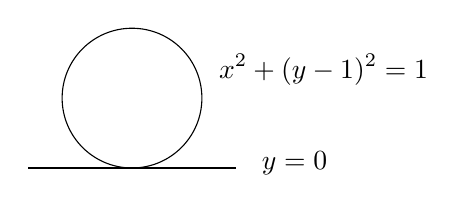
\begin{tikzpicture}[x=0.75pt,y=0.75pt,yscale=-1,xscale=1]
			%uncomment if require: \path (0,300); %set diagram left start at 0, and has height of 300
			
			%Straight Lines [id:da9022525264933119] 
			\draw    (44,106) -- (144,106) ;
			%Shape: Circle [id:dp5620106547865036] 
			\draw   (60.33,72.33) .. controls (60.33,53.74) and (75.41,38.67) .. (94,38.67) .. controls (112.59,38.67) and (127.67,53.74) .. (127.67,72.33) .. controls (127.67,90.93) and (112.59,106) .. (94,106) .. controls (75.41,106) and (60.33,90.93) .. (60.33,72.33) -- cycle ;
			
			% Text Node
			\draw (155.33,97) node [anchor=north west][inner sep=0.75pt]   [align=left] {$\displaystyle y=0$};
			% Text Node
			\draw (134.67,50) node [anchor=north west][inner sep=0.75pt]   [align=left] {$\displaystyle x^{2} +( y-1)^{2} =1$};
		\end{tikzpicture}
	\end{center}
	
	直观上, 直线与圆相切, 两者在相切处有一条公共的 ``无穷小线段''. 更一般地, 任意两条相切的曲线都有一条公共的形如 $D$ 的无穷小线段, 这便是两条曲线共同的切向量.
\end{example}

\paragraph{Kock--Lawvere 公理与导数}

~

\begin{axiom}
	[label={Kock--Lawvere-D}]
	{(Kock--Lawvere 公理)}
	对任意映射 $f \colon D \to R$, 存在唯一的 $a,b\in R$,
	使得
	$$
	f(d) = a + d\cdot b,\quad\forall d\in D.
	$$
	换言之, 作为 $R$-代数有
	$$
	\operatorname{Hom}(D,R) \simeq R[x]/(x^2).
	$$
\end{axiom}

Kock--Lawvere 公理反映了如下的直观: $R$ 上的一个函数在一个很小的邻域上近乎是一次函数.
由此, 我们立刻得到如下的推论.

\begin{propdef}
	{(导函数)}
	对任意函数 $f\colon R\to R$, 存在唯一的函数 $f' \colon R \to R$ 满足
	$$
	f(x+d) = f(x) + d \cdot f'(x),\quad \forall x\in R\,\forall d\in D.
	$$
	称 $f'$ 为 $f$ 的\emph{导函数}. 归纳地定义 $k$ 阶导数 $f^{(k)}(x)$.
\end{propdef}

也就是说, 综合微分几何要求任何函数 $R\to R$ 都是任意次可导的.

\paragraph{Weil 代数与无穷小几何对象}

~

无穷小线段 $D$ 对应代数 $R[x]/(x^2)$. 一般地, 在代数--几何对偶中与无穷小几何对象相对应的代数是 $R$ 上的 \emph{Weil 代数}\footnote{Weil 代数有两种含义, 这里所说的不是来自 Lie 代数的那种 Weil 代数.}.
\begin{definition}
	[label={SDG-Weil-algebra}]
	{(Weil 代数)}
	Weil 代数是形如 $W = R \oplus J$ 的 $R$-代数,
	其中 $J$ 是有限生成自由 $R$-模,
	且为幂零理想. 等价地,
	$$
	W = R[x_1,\cdots,x_n]/I,
	$$
	且存在正整数 $N$ 使得 $x_i^N \in I\,(i=1,\cdots,n)$.
\end{definition}

\begin{remark}
	{}
	上面的概念在 ``经典数学'' (经典逻辑) 中对应\emph{局部 Artin 代数}, 其中 Artin 代数是指不存在无限的理想下降链 (这称为\emph{下降链条件}) 的代数.
	设 $k$ 为域, $A$ 是局部 Artin $k$-代数, $\mathfrak m$ 是 $A$ 的唯一极大理想, 并且额外假设 $k \to A/\mathfrak m$ 是同构.%其剩余域 (residue field).
	可以证明\footnotemark $A \simeq k\oplus\mathfrak m$, $\mathfrak m$ 是有限维 $k$-线性空间且为幂零理想. 定义 \ref{SDG-Weil-algebra} 即是这个结果的类比.
	
	局部 Artin 环在代数几何的形变理论中有重要作用, 这正是因为它对应无穷小几何对象.
\end{remark}

\footnotetext{由中山 (Nakayama) 引理以及下降链条件可得 $\mathfrak m$ 幂零; 又由下降链条件可得每个 $\mathfrak m^j / \mathfrak m^{j+1}$ 是有限维 $k$-线性空间, 从而 $A$ 是有限维 $k$-线性空间.}

\begin{definition}
	{(Weil 代数的谱)}
	对于 Weil 代数 $W$, 定义 $W$ 的\emph{谱}为 $R$-代数同态的空间
	$$
	\operatorname{Spec}W = \operatorname{Hom}_{R\mathsf {Alg}}(W,R),
	$$
	称之为\emph{无穷小几何对象}.
\end{definition}

\begin{example}
	{(常见的无穷小几何对象)}
	\begin{itemize}
		\item 点 $$\text{pt} \simeq \{x\in R\mid x=0\} = \operatorname{Spec} R;$$
		\item 无穷小线段的平方 $$D^2 \simeq \{(x,y)\in R^2 \mid x^2=y^2=0\} = \operatorname{Spec}R[x,y]/(x^2,y^2);$$
		\item $R^2$ 上原点的一阶无穷小邻域 $$D(2) := \{(x,y)\in R^2\mid x^2=xy=y^2=0\} = \operatorname{Spec}R[x,y]/(x^2,xy,y^2);$$
		\item 高阶无穷小邻域
		$$
		D_k := \{x\in R\mid x^{k+1}=0\} = \operatorname{Spec}R[x]/(x^{k+1})\, (k=1,2,3,\cdots).
		$$
	\end{itemize}
\end{example}

前面介绍的 Kock--Lawvere 公理可表述为 $\operatorname{Hom}(\operatorname{Spec}R[x]/(x^2),R) \simeq R[x]/(x^2)$. 类似地有如下公理.

\begin{axiom}
	{(Kock--Lawvere 公理)}
	对于 Weil 代数 $W$, 有
	$$
	\operatorname{Hom}(\operatorname{Spec}W,R)\simeq W.
	$$
\end{axiom}

\begin{remark}
	{(Weil 代数与 Kock--Lawvere 公理的直观)}
	设 $W=R\oplus J$ 是 Weil 代数. 投影 $W \to R$ 对应点 $\text{pt}$ 到无穷小几何对象 $\operatorname{Spec}W$ 的\emph{原点}的嵌入 $$\text{pt} = \operatorname{Spec} R \to \operatorname{Spec}W.$$
	Kock--Lawvere 公理说的是 Weil 代数 $W$ 等同于 $\operatorname{Spec}W$ 上的函数代数. 投影 $W\to R$ 可视为 $\operatorname{Spec}W$ 上的函数在原点处取值; 理想 $J$ 是投影 $W\to R$ 的核, 可视为在原点取值为 $0$ 的函数的集合.
	要求 $J$ 为\emph{幂零}理想, 也即要求在原点取值为 $0$ 的函数都幂零, 直观上说明 $\operatorname{Spec}W$ 是 ``无穷小'' 的.
\end{remark}

Lawvere 以如下的性质刻画无穷小几何对象.

\begin{definition}
	{(无穷小对象, 奇妙右伴随)}
	对于空间 $S$, 若 $(-)^S$ 有右伴随, 则称 $S$ 为\emph{无穷小对象}. 记该右伴随为 $(-)_S$, 称之为\emph{奇妙右伴随} (amazing right adjoint).
\end{definition}

\begin{example}
	{}
	在集合范畴 $\mathsf {Set}$ 中, 只有终对象 $1$ 是无穷小对象.
\end{example}

\begin{remark}
	[label={infinitesimal-object-intuition}]
	{}
	回忆对\topos{}中任意对象 $S$, $(-)^S$ 都有左伴随 $(-)\times S$, 而 $(-)^S$ 有右伴随是非常稀奇的事情. 重要的是此时 $(-)^S$ \emph{保持余极限}. 一个直观如下. 设空间 $X$ 被一族空间 $U_i$ 覆盖 ($X$ 可写成 $U_i$ 和 $U_i\times_X U_j$ 的某种余极限), 那么 $X^S$ 也被 $U_i^S$ 覆盖, 即 $S$ 到 $X$ 的任何映射都必须穿过某个 $U_i$; 这是 $S$ 的像 ``太小'' 导致的.
	
	类似的性质在不是\topos{}的范畴中也有用处. 例如 Abel 群范畴 $\mathsf {Ab}$ 中, 函子 $\operatorname{Hom}(A,{-})$ 保持余极限当且仅当 $A$ 是有限生成投射 $\mathbb{Z}$-模, 这也是一种 ``小'' 的性质.
	
	%映射 $X^D \to Y$ 等同于映射 $X \to Y_D$
\end{remark}

\todo{使用 SDG 的例子, 如 Riemann 曲率}

\todo{无穷小对象的定义, amazing right adjoint}

\subsection{综合微分几何的模型}

本小节介绍综合微分几何的一些模型. 相对简单的模型就能实现 Kock--Lawvere 公理; 而为了使模型满足更多的公理, 以及更加贴近传统的微分几何 (更加 ``有用''), 我们就需要作越来越复杂的调整.
构造综合微分几何模型的贯穿始终的思想是\emph{代数--几何对偶}.

\subsubsection{``代数'' 模型}

首先考虑一个最简单的模型.
\begin{definition}
	[label={SDG-algebraic-model}]
	{}
	考虑有限表现仿射 $\mathbb{R}$-概形范畴 $\mathbb{R}\mathsf{Alg}_{\text{fp}}^\op$.
	回忆, 有限表现 $\mathbb{R}$-代数即形如 $\mathbb{R}[x_1,\cdots,x_n]/(f_1,\cdots,f_m)$ 的代数; 对于有限表现 $\mathbb{R}$-代数 $A$, 以 $\operatorname{Spec} A$ 表示其在对偶范畴中的化身.
	
	所谓\emph{代数模型} (algebraic model) 是 $\mathbb{R}\mathsf{Alg}_{\text{fp}}^\op$ 上的层\topos{} $$\mathsf {Fun}(\mathbb{R}\mathsf{Alg}_{\text{fp}},\mathsf {Set}).$$
\end{definition}

\begin{definition}
	{(直线)}
	定义 \emph{直线}
	$$
		R
		:=\yo(\operatorname{Spec}\mathbb{R}[x]).
	$$
\end{definition}

\begin{remark}
	{}
	这里考虑的\topos{}是 $\mathbb{R}$-代数的\emph{分类\topos{}}, 而 $R$ 是其中的\emph{一般 $\mathbb{R}$-代数} (generic $\mathbb{R}$-algebra).
	
	这些结论对有限生成 $\mathbb{R}$-代数范畴同样成立.
\end{remark}

注意到对 $A\in\mathbb{R}\mathsf {Alg}_{\text{fp}}$,
$$
R(A)=\operatorname{Hom}_{\mathbb{R}\mathsf{Alg}_{\text{fp}}^\op}(\operatorname{Spec}A,\operatorname{Spec}\mathbb{R}[x]) = \operatorname{Hom}_{\mathbb{R}\mathsf {Alg}_{\text{fp}}}(\mathbb{R}[x],A) \simeq A\text{ (作为集合)},
$$
我们发现, $R$ 正是代数范畴到集合范畴的遗忘函子
$$
R\simeq \text{遗忘}
\colon \mathbb{R}\mathsf{Alg}_{\text{fp}} \to \mathsf {Set}.
$$
因此, 使用米田方法, 我们就得到
\begin{prop}
	{}
	$R$ 是交换环.
\end{prop}

有了 $R$, 我们考虑 ``由方程定义的子流形''
$$
M = \{(x_1,\cdots,x_n)\in R^n\mid f_1=\cdots=f_m=0\},
$$
其中 $f_1,\cdots,f_m\in \mathbb{R}[x_1,\cdots,x_n]$ 是多项式. 其范畴语义为拉回
% https://q.uiver.app/#q=WzAsNCxbMSwxLCJSXm0iXSxbMCwxLCJSXm4iXSxbMSwwLCIwIl0sWzAsMCwiTSJdLFsxLDAsIihmXzEsXFxjZG90cyxmX20pIiwyXSxbMywxXSxbMywyXSxbMiwwXV0=
\[\begin{tikzcd}[ampersand replacement=\&]
	M \& 0 \\
	{R^n} \& {R^m,}
	\arrow["{(f_1,\cdots,f_m)}"', from=2-1, to=2-2]
	\arrow[from=1-1, to=2-1]
	\arrow[from=1-1, to=1-2]
	\arrow[from=1-2, to=2-2]
\end{tikzcd}\]
对应 $\mathbb{R}\mathsf {Alg}$ 中的推出
% https://q.uiver.app/#q=WzAsNCxbMSwxLCJcXG1hdGhiYntSfVt5XzEsXFxjZG90cyx5X21dIl0sWzAsMSwiXFxtYXRoYmJ7Un1beF8xLFxcY2RvdHMseF9uXSJdLFsxLDAsIlxcbWF0aGJie1J9Il0sWzAsMCwiTSJdLFswLDEsIihmXzEsXFxjZG90cyxmX20pIl0sWzEsM10sWzIsM10sWzAsMl1d
\[\begin{tikzcd}[ampersand replacement=\&]
	? \& {\mathbb{R}} \\
	{\mathbb{R}[x_1,\cdots,x_n]} \& {\mathbb{R}[y_1,\cdots,y_m],}
	\arrow["{y_i\mapsto f_i}", from=2-2, to=2-1]
	\arrow[from=2-1, to=1-1]
	\arrow[from=1-2, to=1-1]
	\arrow[from=2-2, to=1-2]
\end{tikzcd}\]
故
$$
M = \yo(\operatorname{Spec}\mathbb{R}[x_1,\cdots,x_n]/(f_1,\cdots,f_m)).
$$

\begin{definition}
	{(直线上原点的一阶无穷小邻域)}
	定义
	$$
	D := \{x\in R\mid x^2=0\} =  \yo\big({\operatorname{Spec}\mathbb{R}[x]/(x^2)}\big).
	$$
\end{definition}

我们验证它满足公理 \ref{Kock--Lawvere-D}, 以外部语言叙述即
\begin{prop}
	{}
	$$
	R^D(A) \simeq  A[x]/(x^2).
	$$
\end{prop}

\begin{proof}
	由预层\topos{}指数对象的构造 (命题 \ref{presheaf-category-exponential} 的证明),
	\begin{align*}
		R^D(A) &= \operatorname{Hom}(\yo(\operatorname{Spec}A)\times D,R)\\
		&\simeq \operatorname{Hom}\big(\yo(\operatorname{Spec}A)\times\yo(\operatorname{Spec}\mathbb{R}[x]/(x^2)),
		\yo(\operatorname{Spec}\mathbb{R}[x])\big)\\
		&\simeq \operatorname{Hom}\big(\yo(\operatorname{Spec}A\times\operatorname{Spec}\mathbb{R}[x]/(x^2)),
		\yo(\operatorname{Spec}\mathbb{R}[x])\big)\\
		&\simeq\operatorname{Hom}_{\mathbb{R}\mathsf{Alg}}(\mathbb{R}[x],A\otimes \mathbb{R}[x]/(x^2))\\
		&\simeq A\otimes \mathbb{R}[x]/(x^2))\simeq A[x]/(x^2) \text{ (作为集合).}
	\end{align*}
	其中用到 $\mathbb{R}$-代数的张量积是 $\mathbb{R}\mathsf{Alg}$ 中的和, 即 $\mathbb{R}\mathsf{Alg}^\op$ 中的积.%; 而 $\yo(A)\times\yo(B) \simeq \yo(A\times B)$.
\end{proof}





\subsubsection{光滑代数}

$\mathbb{R}$-代数上的运算是多项式运算; 若将多项式运算扩充为全体 ``光滑'' 运算, 则可产生一个更接近微分几何的模型.

\begin{definition}
	{(光滑代数)}
	\emph{光滑代数} ($C^\infty$-代数) 是指满足如下条件的集合 $A$: 对每个非负整数 $n$ 与每个 $n$ 元光滑函数 $f\in C^\infty (\mathbb{R}^n,\mathbb{R})$ 都有一个 $n$ 元运算, 称为\emph{光滑运算} $A(f)\colon A^n\to A$,
	使得 $f\mapsto A(f)$ 保持复合, 即对于 $h = g \circ (f_1,\cdots,f_k)$, 有
	$$A(h) = A(g) \circ (A(f_1),\cdots,A(f_k)).$$ 换言之, 光滑代数是 Lawvere 理论 $\mathsf {CartSp}$ 的模型 (例 \ref{Lawvere-theory-CartSp}). 光滑代数的同态是保持所有光滑运算的映射. 记光滑代数的范畴为 $C^\infty\mathsf{Alg}$.
\end{definition}

\begin{remark}
	[label={remark-smooth-algebra-R-algebra}]
	{}
	如上定义的 $C^\infty$-代数首先是 $\mathbb{R}$-代数: 考虑 $0$ 元函数 $\mathbb{R}^0\to \mathbb{R}$ 就得到了常量 $A^0\to A$,
	考虑加法与乘法函数 $+,\times\colon \mathbb{R}^2\to \mathbb{R}$ 就得到 $A$ 上的加法与乘法, 考虑映射 $\mathbb{R}^3\to \mathbb{R}, (x,y,z)\mapsto x(y+z) = xy+xz$, 使用 $f\mapsto A(f)$ 保持复合的条件, 就得到 $A$ 上的分配律, 如此这般.
\end{remark}

\begin{example}
	{}
	设 $M$ 是光滑流形, 那么 $M$ 上的光滑函数空间 $C^\infty (M)$ 构成光滑代数: 对 $f\in C^\infty (\mathbb{R}^n,\mathbb{R})$, 定义 $A(f)(f_1,\cdots,f_n)=f\circ (f_1,\cdots,f_n)$.
\end{example}

\begin{example}
	{}
	$\mathbb{R}[\varepsilon]/(\varepsilon^2)$ 是光滑代数: 对 $f\in C^\infty (\mathbb{R}^n,\mathbb{R})$, 定义 $$
	A(f)(a_1+b_1 \varepsilon,\cdots,a_n+b_n \varepsilon)
	=f(a_1,\cdots,a_n)
	+\sum_i \frac{\partial f}{\partial x_i}\Big|_{(a_1,\cdots,a_n)} b_i \varepsilon.$$
	$\mathbb{R}[\varepsilon]/(\varepsilon^2)$ 可视为 ``无穷小线段上的光滑函数空间''.
\end{example}

\begin{example}
	{}
	光滑流形上一点处的光滑函数芽 (定义 \ref{germ-and-stalk}) 构成光滑代数.
\end{example}

%\todo{使用一般 Lawvere 代数中有限生成的概念}
%我们需要有限生成 $C^\infty$-代数的概念.
类比于 $\mathbb{R}[x_1,\cdots,x_n]$ 是 $n$ 个元素生成的自由 $\mathbb{R}$-代数 (交换含幺代数), 有如下命题.

\begin{prop}
	[label={freely-generated-smooth-algebra}]
	{}
	$C^\infty (\mathbb{R}^n)$ 是 $n$ 个元素生成的\emph{自由光滑代数}.
\end{prop}

\begin{proof}
	要证明的是对任意光滑代数 $A$ 与任意 $n$ 个元素 $a_1,\cdots,a_n \in A$,
	存在唯一的同态 $\varphi\colon C^\infty (\mathbb{R}^n) \to A$ 将每个坐标函数 $x_i$ 映射到 $a_i$.
	由定义, 对任意 $f\in C^\infty (\mathbb{R}^n)$,
	$\varphi$ 必须把 $f = f\circ (x_1,\cdots,x_n)$ 映射到 $f(a_1,\cdots,a_n)$, 这便唯一确定了 $\varphi$; 而它确实将投影 $x_i$ 映射到 $a_i$: $x_i(a_1,\cdots,a_n) = a_i$.
\end{proof}

\newcommand{\locus}{处所}

%\todo{有限表现 vs 有限生成}

类比于\fm{}与位象的关系, 以及环与仿射概形的关系, 我们作如下的定义. 其中记号遵循 Moerdijk 与 Reyes \cite{MSIA}.

\begin{definition}
	{(光滑\locus{})}
	定义\emph{光滑\locus{}} (smooth locus, 复数 loci) 的范畴 $\mathbb L$ 为有限生成光滑代数范畴的对偶,
	$$
	\mathbb L:= C^\infty \mathsf {Alg}_{\text{fg}}^{\op},
	$$
	对于光滑代数 $A$,
	记 $\ell A$ 为 $A$ 在对偶范畴中的化身.
\end{definition}

我们发现\topos{} $\widehat {\mathbb L} = \mathsf {Fun}(C^\infty \mathsf {Alg}_{\text{fg}},\mathsf {Set})$ 是综合微分几何某种意义上的模型 (不过它尚且缺少一些微分几何关心的性质).

\begin{definition}
	{}
	定义\emph{直线}
	$$
	R := \yo(\ell C^\infty(\mathbb{R})).
	$$
\end{definition}


\section{量子理论与 Bohr 意象}

\philoquote{A description of physical reality is made in terms of two sets of objects: observables and states.}{Ludwig Faddeev, \emph{Elementary Introduction to Quantum Field Theory }}

对于经典力学与量子力学系统, 最核心的对象是其中的\emph{状态}与\emph{可观测量}.
量子理论有多种不同的公理化. 粗略地说, 我们考虑的一个量子系统由一个 $C^*$-代数 $\mathcal A$ 表示, 可观测量是这个 $C^*$-代数中的自伴元素, 而系统的状态是这个代数到 $\mathbb{C}$ 的某种映射 $$\rho\colon \mathcal A \to \mathbb{C}.$$ 人们常常以一个 Hilbert 空间 $H$ 表示系统中的纯态 (pure states), 而可观测量则被表示为 $H$ 上的自伴算子, 即有表示 $$\pi\colon \mathcal A \to \operatorname{End}(H).$$ 纯态 $\psi\in H$ 对应的映射则是
$$
\rho\colon A\mapsto \langle\psi | A | \psi \rangle := \langle\psi,\pi(A)\psi\rangle,
$$
它给出状态 $\psi$ 下可观测量 $A$ 的 ``期望值''.

\subsection{$C^*$-代数, 经典语境与 Bohr 景}

\begin{definition}
    {($C^*$-代数)}
    \emph{$C^*$-代数}是 $\mathbb{C}$ 上的 Banach 代数 $\big(\mathcal A,\|{-}\|\big)$,
    带有 ``伴随'' 运算 $(-)^*\colon \mathcal A \to \mathcal A$,
    满足对任意 $x\in \mathcal A$,
    \begin{multicols}
    	{2}
    	\begin{itemize}
    		\item $(a^*)^*=a$,
    		\item $(ab)^*=b^*a^*$,
    		\item $(\lambda a)^*=\bar\lambda a^*\,(\lambda\in\mathbb{C})$,
    		\item $\|a^* a\|=\|a\|\|a^*\|=\|a\|^2$.
    	\end{itemize}
    \end{multicols}
    $C^*$-代数的 $*$-子代数是指关于 $(-)^*$ 封闭的子代数.
\end{definition}

\begin{example}
    {}
    对于 Hilbert 空间 $H$, $H$ 上的有界线性算子的代数 $\mathcal B(H)$ 是 $C^*$-代数, 其中 $a^*$ 是 $a$ 的伴随算子. 事实上, 每个 $C^*$-代数都同构于某个形如 $\mathcal B(H)$ 的代数的 $*$-子代数, 因此后者也可作为 $C^*$-代数的一种具体定义.
\end{example}

\begin{definition}
	{(量子力学系统, 可观测量)}
	\begin{itemize}
		\item 一个\emph{量子力学系统} (quantum mechanical system) 是一个 $C^*$-代数 $\mathcal A$;
		\item 系统中的\emph{可观测量} (observable) 是 $\mathcal A$ 中的自伴元素, 即满足 $a^*=a$ 的元素;
		\item 系统中的\emph{状态} (state) 是线性函数 $\rho\colon \mathcal A\to \mathbb{C}$, 满足
		\begin{itemize}
			\item (正性) $\rho(aa^*)\geq 0$;
			\item (归一性) $\rho(1)=1$.
		\end{itemize}
	\end{itemize}
\end{definition}

我们给出经典力学系统的一种定义. 注意经典与量子系统的相似性.

\begin{definition}
	{(Poisson 代数)}
	\emph{Poisson 代数}是 $\mathbb{R}$ 上的含幺交换结合代数 $\mathcal A$ 配备一个运算 $\{-,-\}\colon \mathcal A\otimes \mathcal A\to \mathcal A$, 称为 \emph{Poisson 括号}, 满足
	\begin{itemize}
		\item $(\mathcal A,\{-,-\})$ 是 Lie 代数;
		\item 对任意 $a\in A$, $\{a,-\}\colon A\to A$ 是导子, 也即 $\{a,xy\}=\{a,x\}y+x\{a,y\}$.
	\end{itemize}
\end{definition}

\begin{example}
	{}
	熟悉经典力学的读者知道, 辛流形 $(X,\omega)$ 上的光滑函数代数 $C^\infty (X)$ 有自然的 Poisson 代数结构: 对 $f\in C^\infty (X)$ 定义向量场 $v_f$ 满足 $\omega(v_f,-) = df$, 则 $\{f,g\}:=\omega(v_f,v_g)$ 给出 $C^\infty (X)$ 上的 Poisson 代数结构.
\end{example}

\begin{definition}
	[label={classical-mechanical-system}]
	{(经典力学系统)}
	\begin{itemize}
		\item 一个\emph{经典力学系统} (classical mechanical system) 是一个 Poisson 代数 $(\mathcal A,\{-,-\})$;
		\item 系统中的\emph{可观测量} (observable) 是 $\mathcal A$ 中的元素;
		\item 系统中的\emph{状态} (state) 是线性函数 $\rho\colon \mathcal A\to \mathbb{R}$, 满足
		\begin{itemize}
			\item (正性) $\rho(a^2)\geq 0$;
			\item (归一性) $\rho(1)=1$.
		\end{itemize}
		\item 系统中的\emph{纯态} (pure state) 是满足上面条件的\emph{代数同态} $\mathcal A\to\mathbb{R}$.
	\end{itemize}
\end{definition}

\begin{example}
	{}
	由定义 \ref{classical-mechanical-system}, 对于辛流形 $(X,\omega)$, $X$ 上的一个点 $p$ 对应一个纯态 $C^\infty (X)\to\mathbb{R},f\mapsto f(p)$.
\end{example}

Heisenberg 不确定性原理表明, 不交换的可观测量不可同时确定, 而一族相交换的可观测量可以同时确定. 因此我们格外关注那些交换的子代数.

\begin{definition}
    {(经典语境)}
    对于量子力学系统 $\mathcal A$, 称 $\mathcal A$ 的一个交换 $*$-子代数为一个\emph{经典语境} (classical context).
    记 $\mathcal C(\mathcal A)$ 为 $\mathcal A$ 的交换 $*$-子代数在包含关系下构成的偏序集.
\end{definition}

\begin{remark}
    {}
    语境这个名字的含义是, 一个可观测量只在某些特定的语境 (也就是包含它的那些语境) 下才有确定的值. 在一个固定的语境中, 可观测量的表现无异于一个经典系统.
\end{remark}

这里我们稍微偏题, 介绍偏序集上的层.

\todo{移到层论那一章}

\begin{definition}
    {(Alexandorff 空间)}
    若一个拓扑空间中开集的任意交仍是开集, 则称其为 \emph{Alexandorff 空间}.
\end{definition}

\begin{definition}
    {(Alexandroff 拓扑)}
    设 $P$ 为偏序集. 定义 $P$ 上的 \emph{Alexandroff 拓扑}是以向上封闭集为开集的拓扑. 其中, 称 $Q\subset P$ 为\emph{向上封闭集}是指对任意 $x\in Q,y\in P$, 若 $x\leq y$, 则 $y\in Q$. 这给出了函子
    \[
    \operatorname{Alex}\colon \mathsf {Poset} \to \mathsf {Top}.
    \]
\end{definition}

\begin{prop}
    {}
    对任意偏序集 $P$, $P$ 上的预层可自然延拓为 $P$ 的 Alexandroff 拓扑上的层.
\end{prop}

% sheaf vs cosheaf
%
%\begin{definition}
%    {(Bohr 景)}
%    范畴, 也称 \emph{Bohr 景}. Bohr 景上的意象将是我们主要的研究对象.
%\end{definition}

\subsection{Bohr 意象}

\begin{definition}
    {(Bohr 意象)}
    称 $\mathcal C(\mathcal A)$ 上的预层意象为 \emph{Bohr 意象}.
\end{definition}

一个量子系统的\emph{状态} (state) 是一个线性映射 $A \to \mathbb{C}$

\begin{definition}
    {(Gelfand 谱)}
    对于交换 $C^*$-代数 $A$, 定义其 \emph{Gelfand 谱}
$$
\Sigma(A) := \{C^*\text{-代数同态}\,\lambda\colon A \to\mathbb{C}\},
$$
其拓扑为使得所有映射 $\Sigma(A)\to\mathbb{C}, \lambda \mapsto \lambda (x)$ 都连续的最弱拓扑. 由 Gelfand--Mazur 定理, Gelfand 谱 $\Sigma(A)$ 也是 $A$ 的极大理想的集合.
\end{definition}

$\Sigma(A)$ 上拓扑的定义旨在保证每个元素 $x\in A$ 都对应 $\Sigma(A)$ 上的一个复值连续函数. 如下定理表明这个对应实际上是一个同构; 这是代数--几何对偶的一例.

\begin{prop}
    {(Gelfand--Naimark 对偶)}
    记 $\mathsf {CC}^*$ 为交换 $C^*$-代数的范畴, $\mathsf{CHaus}$ 为紧 Hausdorff 空间的范畴,
    那么 Gelfand 谱给出反变函子 $\Sigma\colon \big(\mathsf {CC}^*\big)^{\op} \to \mathsf {CHaus}$, 且有范畴等价
    \[\begin{tikzcd}[ampersand replacement=\&]
    	{\big(\mathsf {CC}^*\big)^{\op}} \& {\mathsf {CHaus},}
    	\arrow["\Sigma", shift left, from=1-1, to=1-2]
    	\arrow["{C({-},\mathbb{C})}", shift left, from=1-2, to=1-1]
    \end{tikzcd}\]
    其中 $C(X,\mathbb{C})$ 是空间 $X$ 上复值连续函数的 $C^*$-代数.
\end{prop}

可观测量代数与状态空间互为对偶. 经典力学中, 可观测量是状态空间上的函数; 反过来, 状态空间上的点可视为可观测量代数到 $\mathbb{R}$ 的代数同态.
完全类似地, 在量子力学中, 给定语境 $A$, 对应的 "状态空间" $\Sigma(A)$ 中的点就是 $A$ 到 $\mathbb{C}$ 的代数同态, 而 $A$ 中的可观测量则可视为状态空间 $\Sigma(A)$ 上的函数.

\begin{definition}
    {(谱预层)}
    对于语境 $A_1 \subset A_2$, 有限制映射 $\Sigma(A_2)\to\Sigma(A_1)$. 这定义了 $\mathcal C(\mathcal A)$ 上的预层 $\Sigma$.
\end{definition}

\begin{remark}
    {}
    预层 $\Sigma$ 整合了所有经典语境的几何信息.
    
    一般而言, 一个可观测量只能给出预层 $\Sigma$ 的局部截面, 而无法给出整体截面.
\end{remark}

Bohr 意象中对象 $\Sigma$ 的构造可视为将 Gelfand 谱的构造由交换代数推广到非交换代数, 成为与交换子代数相对偶的空间的系统. 它实际上是 Bohr 意象中的内蕴位象 (internal locale). 而交换子代数的全体构成 Bohr 意象中的一个\emph{内蕴代数}. 由此, Bohr 意象的内语言允许我们像谈论经典态一样谈论量子态.

\subsection{Bohr 意象中的命题}



在一个经典系统中, 命题是状态空间的子集, 表示这个命题在何种状态下成立.
类似地, 量子系统中的命题是预层意象中 $\Sigma$ 的子对象, 或称子函子.

\section{Cohen 力迫法}

\label{Cohen-forcing}

1874 年, Georg Cantor 证明了自然数与实数 (又称连续统) 之间不存在一一对应\footnote{不过他的第一个证明并非现在流行的对角线论证.}. Cantor 接着于 1878 年提出了\emph{连续统假设} (continuum hypothesis),
$$
\fbox{在自然数集合 $N$ 与连续统 $PN$ 之间不存在其它的基数.}
$$

1940 年, Kurt G\"odel 证明连续统假设与 Zermelo--Fraenkel 集合论相容. 1963 年, Paul Cohen 证明了连续统假设独立于带有选择公理的 Zermelo--Fraenkel 集合论 (ZFC), 即 ZFC 既不能证明, 也不能证伪连续统假设.

% Boole 意象的内容放在了第一章末尾.

在 \ref{Boolean-topos} 节我们介绍了 Boole \topos{}. 我们可以在这样的\topos{}中做 ``经典数学''. 下面的内容本质上等同于 Cohen 证明连续统假设独立于 ZFC 所使用的方法, 只不过翻译到了\topos{}的语境.

\begin{prop}
	{}
	存在一个 Boole \topos{}, 其中选择公理成立, 而连续统假设不成立.
\end{prop}

\subsubsection{基础知识}

回忆任何\topos{}上都有一个 Lawvere--Tierney 拓扑 $\neg\neg$. 有趣的是, 它总是给出一个 Boole 意象.

\begin{prop}
	{}
	对任意\topos{} $\mathcal C$, $\operatorname{Sh}_{\neg\neg}\mathcal C$ 为 Boole \topos{}.
\end{prop}
\begin{proof}
	由 Boole \topos{}的内语言刻画 (\ref{internal-Boolean-topos}), 我们要在 $\operatorname{Sh}_{\neg\neg}\mathcal C$ 中证明 $\forall p\in\Omega (p\lor \neg p)$.
	% 需要几何态射在命题上的作用
	\todo{}
\end{proof}

\begin{definition}
	{(基数的比较)}
	对于一个\topos{}中的两个对象 $X,Y$, 若存在单射 $X\to Y$, 且 $\operatorname{Epi}(X,Y)\simeq 0$, 则称 $X$ 的基数小于 $Y$, 记为 $X<Y$.
\end{definition}

回忆 $\operatorname{Epi}(X,Y)$ 的定义 (\ref{set-of-epimorphisms}), $\operatorname{Epi}(X,Y)\simeq 0$ 当且仅当公式 $\forall f\in Y^X\,\neg(\operatorname{im}f = Y)$ 成立.



\section{凝聚态数学}

% 【潜水】岩豚鼠: 我们要解决拓扑abel群范畴不是abel范畴的问题, 首先要解决拓扑空间范畴中连续双射不可逆的问题. 注意到紧Hausdorff空间没有这个问题, 我们就尝试将一般的拓扑空间换成紧Hausdorff空间范畴上的层, 而这个景有一族基叫做投射有限集. 这里的拓扑是取连续满射为覆盖. 每个紧Hausdorff空间都被它自己的集合作为离散空间覆盖, 注意到紧Hausdorff空间到一般拓扑空间范畴的嵌入有个左伴随叫Stone—Cech紧化, 我们就可以把基取为离散空间的SC紧化.
